\documentclass[letter,11pt]{article}

\usepackage[spanish,es-nodecimaldot]{babel}
\usepackage[utf8]{inputenc}

\usepackage{lmodern}
\usepackage[T1]{fontenc}
\usepackage{textcomp}

\usepackage{framed}
\usepackage[svgnames]{xcolor}
\colorlet{shadecolor}{Gainsboro!50}

\usepackage[labelfont=bf]{caption}
\usepackage{graphicx}
\usepackage{pstricks}

\usepackage{anysize}
\marginsize{3cm}{2cm}{2cm}{3cm}

\usepackage{url}
\usepackage{siunitx}
\usepackage{amsmath}
\usepackage{array}
\usepackage{alltt}

\usepackage{caption}
\newcommand{\source}[1]{\vspace{-11pt} \caption*{\small{\textbf{Fuente:} {#1}}}}

\usepackage{fancyhdr}
\usepackage{lastpage}
\pagestyle{fancy}
\fancyhf{}
\fancyhead[LE,RO]{Laboratorio de Física Básica II}
\fancyfoot[CO,CE]{\thepage\ de \pageref{LastPage}}

\special{papersize=215.9mm,279.4mm}

\usepackage[
    pdfauthor={Carlos Eduardo Caballero Burgoa},%
    pdftitle={Laboratorio de Física Básica II},%
    pdfsubject={Péndulo simple},%
    colorlinks,%
    citecolor=black,%
    filecolor=black,%
    linkcolor=black,%
    urlcolor=black,
    breaklinks]{hyperref}
\usepackage{breakurl}

\newcommand{\blankpage}{
\newpage
\thispagestyle{empty}
\mbox{}
\newpage
}

\renewcommand{\arraystretch}{1.2}

\title{Informe 3: Péndulo simple}
\author{Carlos Eduardo Caballero Burgoa \\
    \small{\href{mailto:200201226@est.umss.edu}{200201226@est.umss.edu}}
}
\date{\today}

\begin{document}

\maketitle
\begin{center}
    \textbf{Grupo}: J2\\
    \textbf{Docente}: Ing. Milka Mónica Torrico Troche\\
    \textbf{Carrera}: Ing. Electromecánica
\end{center}

\begin{abstract}
    Este documento detalla el experimento realizado en simulador para hallar 
    la relación funcional entre el periodo de oscilación ($T$) y la longitud
    ($L$) de un péndulo simple, además de calcular el valor de la aceleración
    de la gravedad; para esto se realizó la medición de 10 oscilaciones de un
    péndulo con una longitud determinada; y posteriormente se calculó la
    relación funcional después de linealizar la cuerva y ajustarla con el método
    de mínimos cuadrados, finalmente se determinó el valor de la gravedad ($g$)
    con su respectivo error.
\end{abstract}

\section{Introducción}

Un péndulo simple es un modelo idealizado que consiste en una masa puntual
suspendida de una cuerda no expansible y de masa despreciable. Si la masa se
mueve a un lado de su posición de equilibrio vertical descendente, oscilará
alrededor de dicha posición \cite{Sears}.

\begin{figure}
\centering
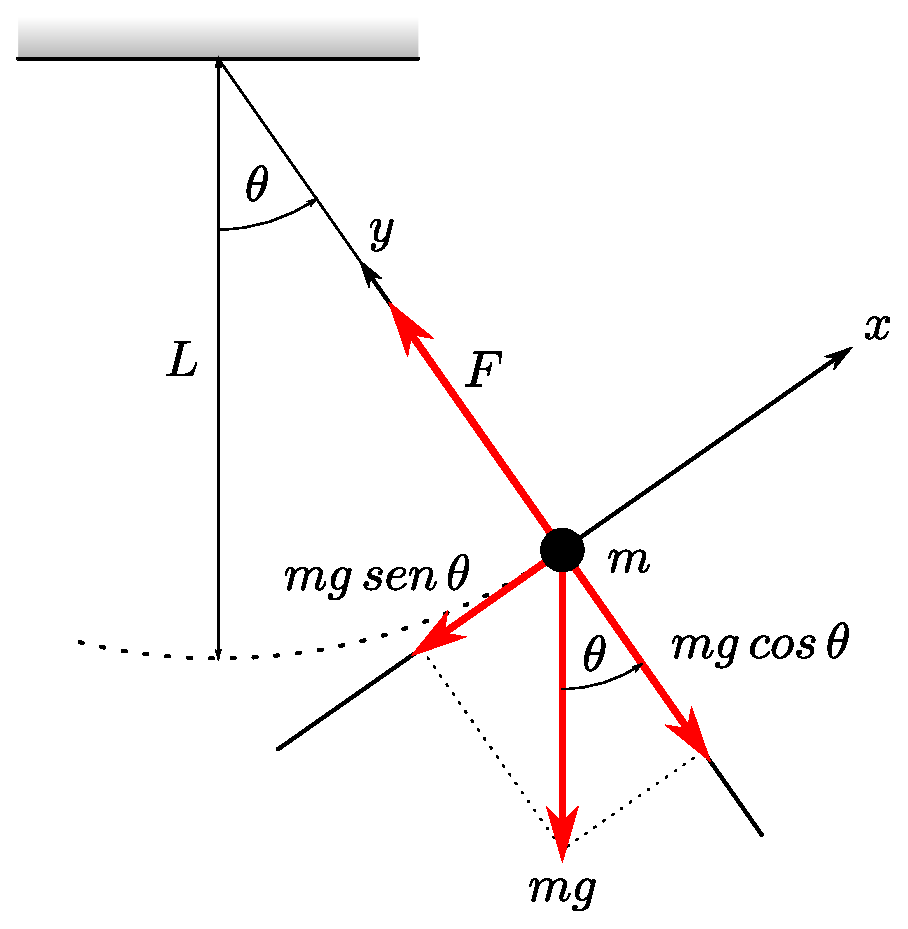
\includegraphics[width=0.38\textwidth]{resources/f1.eps}
\caption{Péndulo simple idealizado.}
\label{figura1}
\source{2013. Sears y Zemansky. Física Universitaria Volumen I. Pagina 454.}
\end{figure}

En la \textbf{Figura \ref{figura1}} se muestran las fuerzas que actúan sobre la
masa ($m$) en cualquier instante del movimiento, estas fuerzas son: La tensión
($F$) de la cuerda y la fuerza de gravedad ($mg$), que se descompone en función
del ángulo desplazado ($\theta$), en una componente normal ($mg\, cos\, \theta$)
y una componente tangencial ($mg\, sen\, \theta$) \cite{GUIA}.

Aplicando la segunda ley de \emph{Newton} en la dirección tangencial, se
obtiene:

\begin{equation*}
    -mg\, sen\, (\theta) = m\, a_t
\label{segundaley}
\end{equation*}
\vspace{-0.16cm}

La aceleración en la dirección tangencial es:

\begin{equation*}
    a_t = \frac{d^2 S}{dt^2}
\end{equation*}
\vspace{-0.16cm}

Donde $S$ es la longitud del arco o trayectoria circular, cuya relación con el
ángulo $\theta$ y la longitud de la cuerda $L$ es:

\begin{equation*}
    S = \theta\, L
\end{equation*}
\vspace{-0.16cm}

Por tanto:

\begin{equation*}
    \frac{d^2 \theta}{dt^2} + \frac{g}{L} sen\, (\theta) = 0
\end{equation*}
\vspace{-0.16cm}

Si consideramos tan solo oscilaciones de pequeña amplitud, de modo que el
ángulo $\theta$ sea siempre suficientemente pequeño, entonces el valor del
$sen\, (\theta)$ será muy próximo al valor de $\theta$ expresado en radianes (
$sen\, (\theta) \cong \theta$, para $\theta$ suficientemente pequeño), como podemos
apreciar en el \textbf{Cuadro \ref{cuadro1}} \cite{WIKI1}, y la ecuación
anterior se reduce a:

\begin{table}[!h]
\begin{center}
\begin{tabular}{|>{\centering}m{0.50cm}<{\centering}
                |>{\centering}m{1.25cm}<{\centering}
                |>{\centering}m{1.25cm}<{\centering}
                |>{\centering}m{1.50cm}<{\centering}|
                |>{\centering}m{0.50cm}<{\centering}
                |>{\centering}m{1.25cm}<{\centering}
                |>{\centering}m{1.25cm}<{\centering}
                |>{\centering}m{1.50cm}<{\centering}|}
\hline
$\theta [^\circ]$ & $\theta [rad]$ & $sen\, \theta$ & Dif. (\%) & $\theta [^\circ]$ & $\theta [rad]$ & $sen\, \theta$ & Dif. (\%) \tabularnewline \hline
 0 & 0.00000 & 0.00000 & 0.00 & 15 & 0.26180 & 0.25882 & 1.15 \tabularnewline \hline
 2 & 0.03491 & 0.03490 & 0.02 & 20 & 0.34907 & 0.34202 & 2.06 \tabularnewline \hline
 5 & 0.08727 & 0.08716 & 0.13 & 25 & 0.43633 & 0.42262 & 3.25 \tabularnewline \hline
10 & 0.17453 & 0.17365 & 0.51 & 30 & 0.52360 & 0.50000 & 4.72 \tabularnewline \hline
\end{tabular}
\caption{Comparación entre el valor de un ángulo (rad) y su seno.}
\label{cuadro1}
\source{Wikipedia: Péndulo simple.}
\end{center}
\end{table}

\begin{equation*}
    \frac{d^2 \theta}{dt^2} + \frac{g}{L} \theta = 0
\end{equation*}
\vspace{-0.16cm}

La ecuación anterior corresponde a un \textbf{oscilador armónico simple} cuya
solución general es:

\begin{equation*}
    \theta(t) = A\, cos\, (\omega\, t + \phi)
\end{equation*}
\vspace{-0.16cm}

Donde $A$ representa el máximo desplazamiento angular de $\theta$, $\omega$ es la
frecuencia angular, y $\phi$ el desfase. Tanto la magnitud $A$, como $\phi$ son
dos constantes determinadas por las condiciones iniciales.

La frecuencia angular ($\omega$) esta determinado por:

\begin{equation*}
    \omega = \sqrt{\frac{g}{L}}
\end{equation*}
\vspace{-0.16cm}

Considerando que $\omega = 2\pi / T$, el periodo de oscilación para el péndulo
simple es:

\begin{equation}
    T = 2\pi\, \sqrt{\frac{L}{g}} = \frac{2\pi}{\sqrt{g}} \sqrt{L}
\label{periodo}
\end{equation}
\vspace{-0.16cm}

Para el experimento se verificará la \textbf{Ecuación \ref{periodo}}, a partir
de la toma de datos del tiempo de oscilación del péndulo para hallar el periodo
($T$) a partir de una longitud de cuerda establecida ($L$). Finalmente se
determinará el valor de la gravedad ($g$) despejándola de la misma ecuación.

\section{Método experimental}

\begin{figure}
\centering
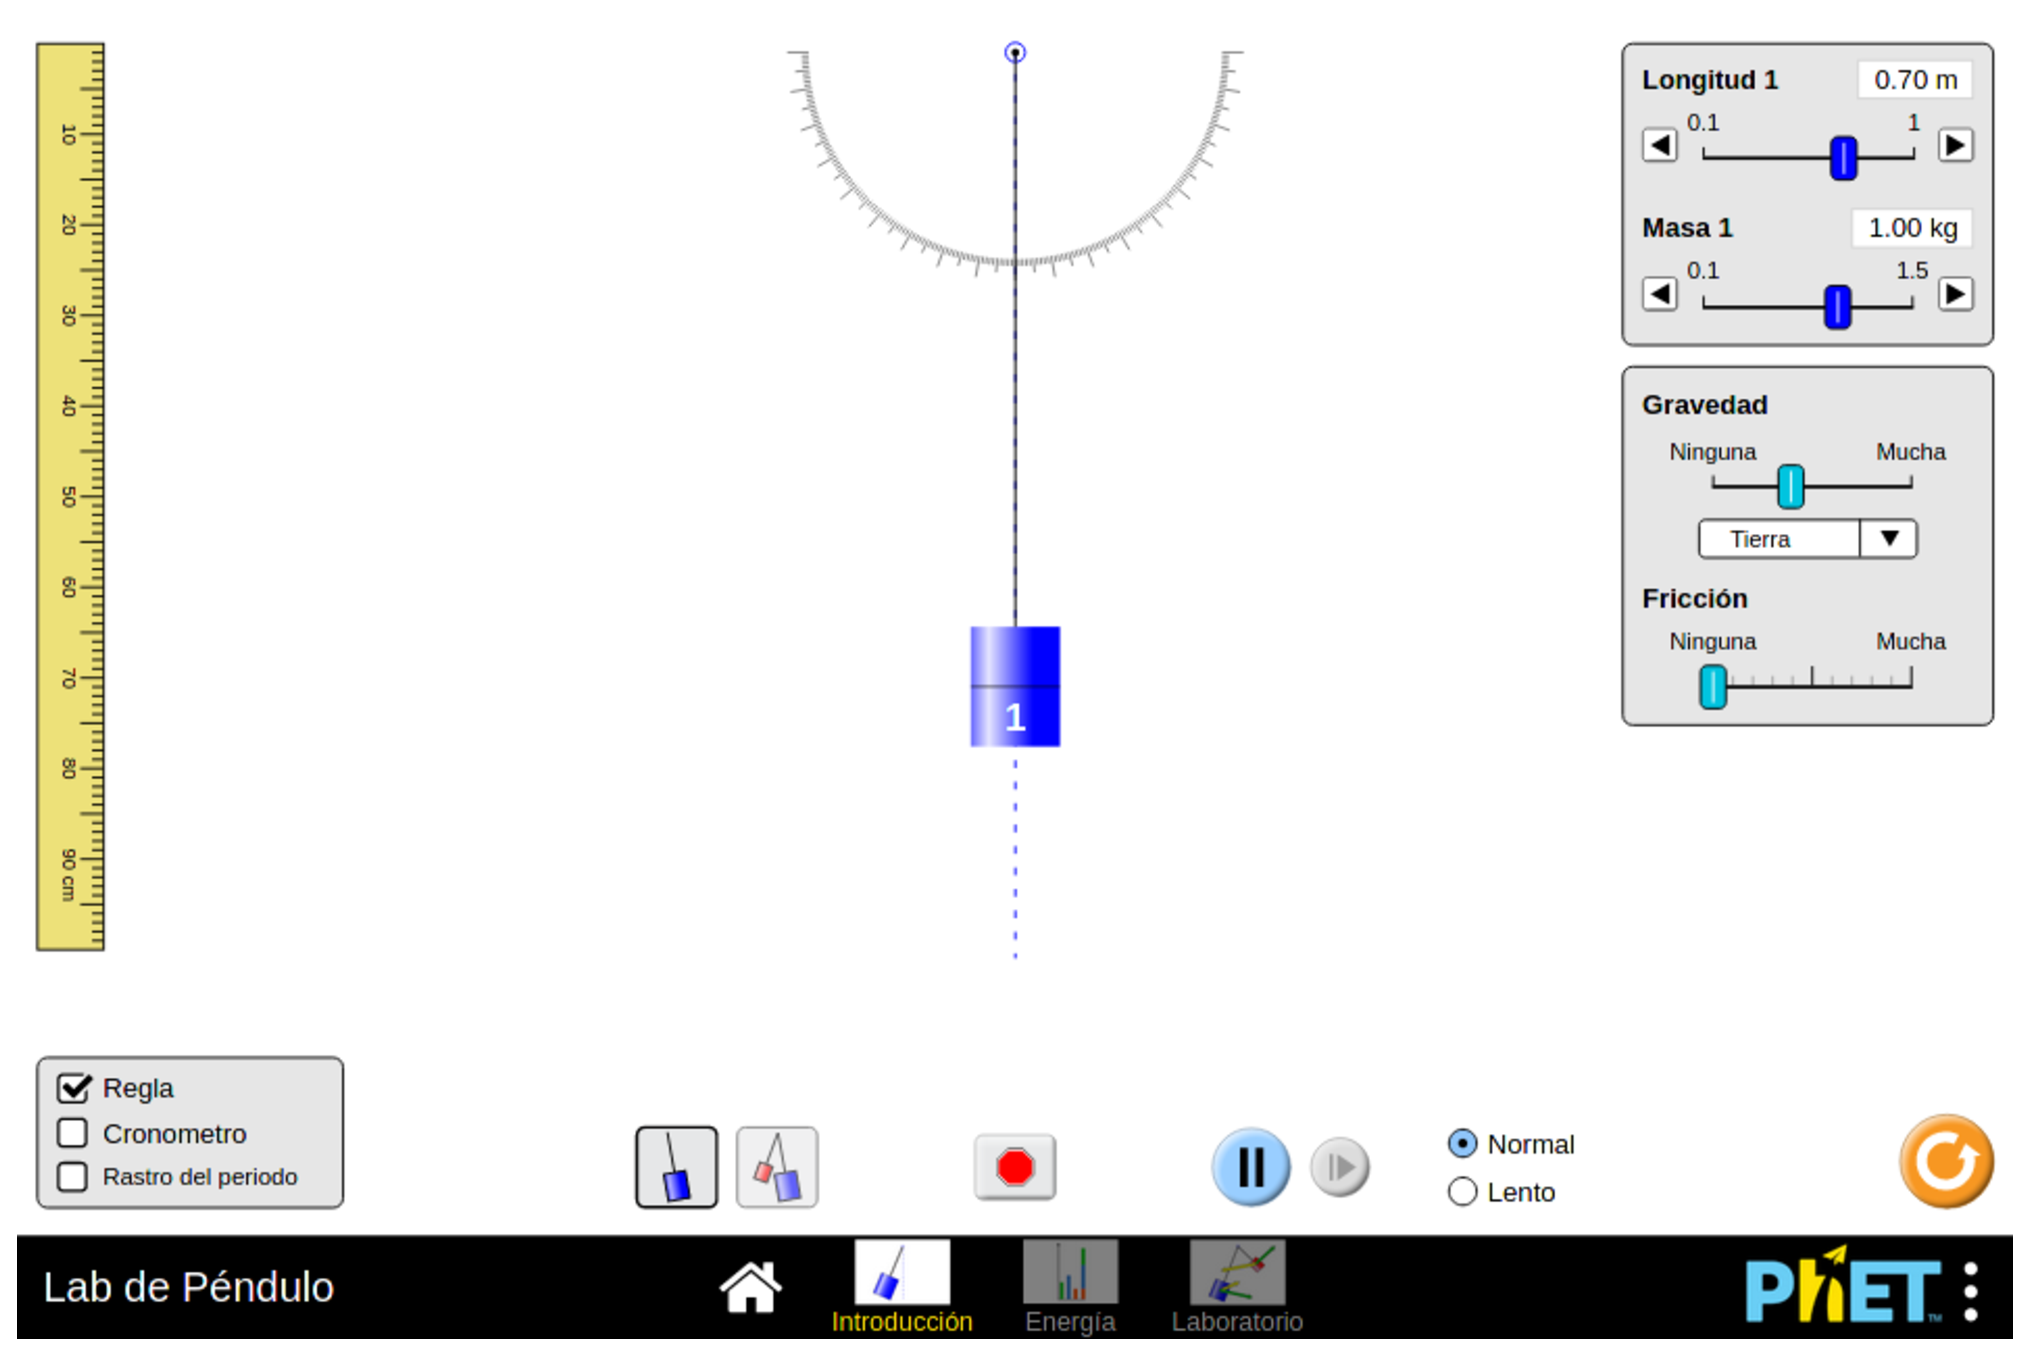
\includegraphics[width=0.90\textwidth]{resources/f2.eps}
\caption{Simulador de péndulo simple.}
\label{figura2}
\source{Fotografía propia.}
\end{figure}

Para la realización del experimento, se utilizará el simulador de péndulo simple
de \emph{PHET}, ubicado en la dirección web:
\url{https://phet.colorado.edu/sims/html/pendulum-lab/latest/pendulum-lab_es.html},
esté se muestra en la \textbf{Figura \ref{figura2}}.

Para el simulador se escoge un valor de longitud ($L$), que se mantendrá
constante durante la medición, y se registrarán 2 veces la cantidad de tiempo
que requiere el péndulo para hacer 10 oscilaciones completas, todas las
mediciones con una inclinación de $8^\circ$.

Una vez medidos los datos para 10 valores distintos de longitud ($L$), se
procederá a calcular el periodo ($T$) con la siguiente ecuación:

\begin{equation}
    T = \frac{\bar{t}}{10}
\label{periodo10}
\end{equation}
\vspace{0.10cm}

Donde $\bar{t}$, es el valor representativo para una serie de mediciones
realizadas.

Luego se procederá a graficar la relación longitud ($L$) vs. periodo ($T$), para
realizar primeramente la linealización de la curva por logaritmos, y luego el
calculo de la recta por el método de los mínimos cuadrados, para posteriormente
hallar la relación funcional entre las variables.

Finalizando con el calculo del valor de la gravedad, a partir de la
\textbf{Ecuación \ref{periodo}}:

\begin{equation*}
    a = \frac{2 \pi}{\sqrt{g}}
\end{equation*}
\begin{equation}
    g = \frac{4 \pi^2}{a^2}
\label{gravedad}
\end{equation}
\vspace{0.10cm}

Donde $a$ es uno de los parámetros de la curva hallada.

\vspace{0.35cm}
\textbf{Datos necesarios para el experimento:} \\

Masa del peso a oscilar por el péndulo:
\begin{equation*}
    m = 1.50 [kg]
\end{equation*}

Precisión de la regla:
\begin{equation*}
    P_L = 0.01 [m]
\end{equation*}

Precisión de la balanza:
\begin{equation*}
    P_m = 0.01 [kg]
\end{equation*}

Precisión del cronometro:
\begin{equation*}
    P_t = 0.01 [s]
\end{equation*}

\section{Resultados}

En el \textbf{Cuadro \ref{cuadro2}}, se pueden ver los valores tomados del 
experimento, tanto la longitud como el tiempo de 10 oscilaciones tomados 2
veces, además del valor del periodo resultante.

\begin{table}[!h]
\begin{center}
\begin{tabular}{|c|>{\centering}m{2.4cm}<{\centering}|
                  |>{\centering}m{2.4cm}<{\centering}
                  |>{\centering}m{2.4cm}<{\centering}|
                  |>{\centering}m{2.4cm}<{\centering}|}
\hline
$i$ & $L_i [m]$ & $t_{1i} [s]$ & $t_{2i} [s]$ & $T [s]$ \tabularnewline \hline
\hline
 1 & 0.55 & 14.85 & 14.81 & 1.4830 \tabularnewline \hline
 2 & 0.60 & 15.42 & 15.45 & 1.5435 \tabularnewline \hline
 3 & 0.65 & 16.09 & 16.14 & 1.6115 \tabularnewline \hline
 4 & 0.70 & 16.88 & 16.76 & 1.6820 \tabularnewline \hline
 5 & 0.75 & 17.35 & 17.37 & 1.7360 \tabularnewline \hline
 6 & 0.80 & 17.87 & 17.92 & 1.7895 \tabularnewline \hline
 7 & 0.85 & 18.37 & 18.41 & 1.8390 \tabularnewline \hline
 8 & 0.90 & 19.01 & 18.94 & 1.8975 \tabularnewline \hline
 9 & 0.95 & 19.53 & 19.62 & 1.9575 \tabularnewline \hline
10 & 1.00 & 20.02 & 19.92 & 1.9970 \tabularnewline \hline
\end{tabular}
\caption{Mediciones de tiempo en función de la longitud del péndulo.}
\label{cuadro2}
\source{Elaboración propia.}
\end{center}
\end{table}

\begin{figure}
\centering
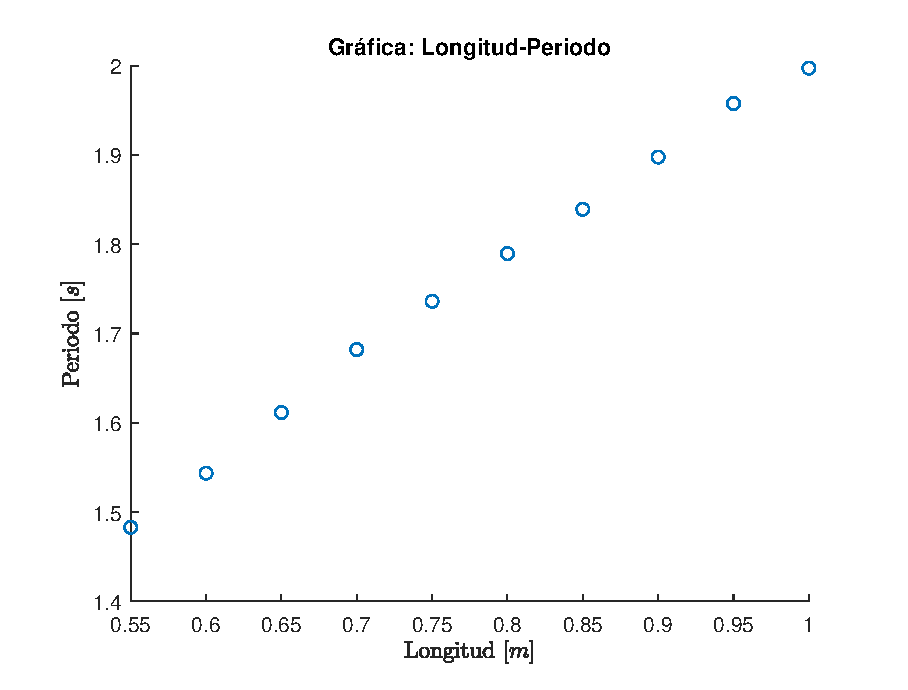
\includegraphics[width=0.80\textwidth]{resources/m1.1.eps}
\caption{Gráfica de longitud vs periodo.}
\label{figura3}
\source{Elaboración propia.}
\end{figure}

A partir de los datos obtenidos se calculó el periodo de oscilación ($T$) para
los valores de longitud ($L$), de los cuales se genera la gráfica de la
\textbf{Figura \ref{figura3}}.

Posteriormente se linealizó la curva por logaritmos, y luego se realizó el ajuste
de la curva, por el método de los mínimos cuadrados, resultando los
siguientes valores, con su coeficiente de correlación ($r$):

\begin{equation*}
    A = (0.6941 \pm 0.0016) [u]; 0.2354 \%
\end{equation*}
\begin{equation*}
    B = (0.5022 \pm 0.0049) [u]; 0.9791 \%
\end{equation*}
\begin{equation*}
    r = 0.9996
\end{equation*}

Con los valores hallados, se procedió a calcular los valores originales
de la curva, resultando:

\begin{equation*}
    a = (2.0019 \pm 0.0033) [s/\sqrt{m}]; 0.1634 \%
\end{equation*}
\begin{equation*}
    b = (0.5022 \pm 0.0049) [u]; 0.9791 \%
\end{equation*}
\vspace{0.10cm}

Resultando el modelo de ajuste:

\begin{equation*}
    T = 2.0019 L^{0.5022}
\end{equation*}
\vspace{0.10cm}

Por tanto la relación funcional entre $T$ y $L$, es:

\begin{equation*}
    T \propto \sqrt{L}
\end{equation*}
\vspace{0.10cm}

Verificándose el comportamiento establecido por la
\textbf{Ecuación \ref{periodo}}.

Para el calculo de la gravedad ($g$) se utiliza la
\textbf{Ecuación \ref{gravedad}}, resultando:

\begin{equation*}
    g = (9.8508 \pm 0.0322) [m/s^2]; 0.3268 \%
\end{equation*}

\section{Discusión}

La gráfica obtenida de la longitud vs. periodo, visualmente aparenta ser una
relación lineal entre las variables, esto se debe al intervalo de la medición
de la longitud $[0.55, 1.00]$, se recomienda tener datos mas dispersos para
evitar una posible confusión de este tipo.

\section{Conclusiones}

Se realizó la gráfica de longitud vs periodo, se linealizó y realizó el ajuste
de la curva por el método de mínimos cuadrados y se halló la relación funcional
entre estas dos variables, confirmándose la ecuación teórica de un oscilador
armónico simple.

También se halló el valor de la gravedad, siendo está la misma que el simulador
establecía.

\begin{thebibliography}{99}

\bibitem{Sears} Sears y Zemansky (2013).\\
Física Universitaria. Volumen 1.\\
13va Edición.\\
Capitulo 11.

\bibitem{GUIA} Departamento de Física - UMSS.\\
Laboratorio de Física Básica II.\\
Guía - Cartilla de laboratorio.\\
Gestión I/2020.

\bibitem{WIKI1} Péndulo simple \\
Extraído el 27 de Abril del 2021, de: \\
\url{https://es.wikipedia.org/wiki/P%C3%A9ndulo_simple}.

\end{thebibliography}

\newpage
\section*{Anexo: Cálculos adicionales}

Conociendo $t_{1i}$, $t_{2i}$, se detallan los valores del valor representativo
($\bar{t}$), y el periodo de oscilación ($T$) en el
\textbf{Cuadro \ref{cuadro3}}.

\begin{table}[!h]
\begin{center}
\begin{tabular}{|c|>{\centering}m{2.5cm}<{\centering}
                  |>{\centering}m{2.5cm}<{\centering}
                  |>{\centering}m{3.4cm}<{\centering}
                  |>{\centering}m{3.4cm}<{\centering}|}
\hline
$i$ & $t_{1i} [s]$ & $t_{2i} [s]$ & $\bar{t} [s]$ & $T [s]$ \tabularnewline \hline
 1 & $(14.85 \pm 0.01)$ & $(14.81 \pm 0.01)$ & $(14.8300 \pm 0.0200)$ & $(1.4830 \pm 0.0020)$ \tabularnewline \hline
 2 & $(15.42 \pm 0.01)$ & $(15.45 \pm 0.01)$ & $(15.4350 \pm 0.0150)$ & $(1.5435 \pm 0.0015)$ \tabularnewline \hline
 3 & $(16.09 \pm 0.01)$ & $(16.14 \pm 0.01)$ & $(16.1150 \pm 0.0250)$ & $(1.6115 \pm 0.0025)$ \tabularnewline \hline
 4 & $(16.88 \pm 0.01)$ & $(16.76 \pm 0.01)$ & $(16.8200 \pm 0.0600)$ & $(1.6820 \pm 0.0060)$ \tabularnewline \hline
 5 & $(17.35 \pm 0.01)$ & $(17.37 \pm 0.01)$ & $(17.3600 \pm 0.0100)$ & $(1.7360 \pm 0.0010)$ \tabularnewline \hline
 6 & $(17.87 \pm 0.01)$ & $(17.92 \pm 0.01)$ & $(17.8950 \pm 0.0250)$ & $(1.7895 \pm 0.0025)$ \tabularnewline \hline
 7 & $(18.37 \pm 0.01)$ & $(18.41 \pm 0.01)$ & $(18.3900 \pm 0.0200)$ & $(1.8390 \pm 0.0020)$ \tabularnewline \hline
 8 & $(19.01 \pm 0.01)$ & $(18.94 \pm 0.01)$ & $(18.9750 \pm 0.0350)$ & $(1.8975 \pm 0.0035)$ \tabularnewline \hline
 9 & $(19.53 \pm 0.01)$ & $(19.62 \pm 0.01)$ & $(19.5750 \pm 0.0450)$ & $(1.9575 \pm 0.0045)$ \tabularnewline \hline
10 & $(20.02 \pm 0.01)$ & $(19.92 \pm 0.01)$ & $(19.9700 \pm 0.0500)$ & $(1.9970 \pm 0.0050)$ \tabularnewline \hline
\end{tabular}
\caption{Calculo del periodo de oscilación.}
\label{cuadro3}
\source{Elaboración propia.}
\end{center}
\end{table}

En el \textbf{Cuadro \ref{cuadro4}}, se detallan los valores logaritmizados de
$T$ y $L$:

\begin{table}[!h]
\begin{center}
\begin{tabular}{|c|>{\centering}m{2.5cm}<{\centering}
                  |>{\centering}m{2.5cm}<{\centering}|}
\hline
$i$ & $ln(L)$ & $ln(T)$ \tabularnewline \hline
 1 & -0.5978 & 0.3941 \tabularnewline \hline
 2 & -0.5108 & 0.4341 \tabularnewline \hline
 3 & -0.4308 & 0.4772 \tabularnewline \hline
 4 & -0.3567 & 0.5200 \tabularnewline \hline
 5 & -0.2877 & 0.5516 \tabularnewline \hline
 6 & -0.2231 & 0.5819 \tabularnewline \hline
 7 & -0.1625 & 0.6092 \tabularnewline \hline
 8 & -0.1054 & 0.6405 \tabularnewline \hline
 9 & -0.0513 & 0.6717 \tabularnewline \hline
10 &       0 & 0.6916 \tabularnewline \hline
\end{tabular}
\caption{Valores logaritmizados de $L$ y $T$.}
\label{cuadro4}
\source{Elaboración propia.}
\end{center}
\end{table}

Los valores del \textbf{Cuadro \ref{cuadro4}}, pueden verse gráficamente en la
figura

\begin{figure}
\centering
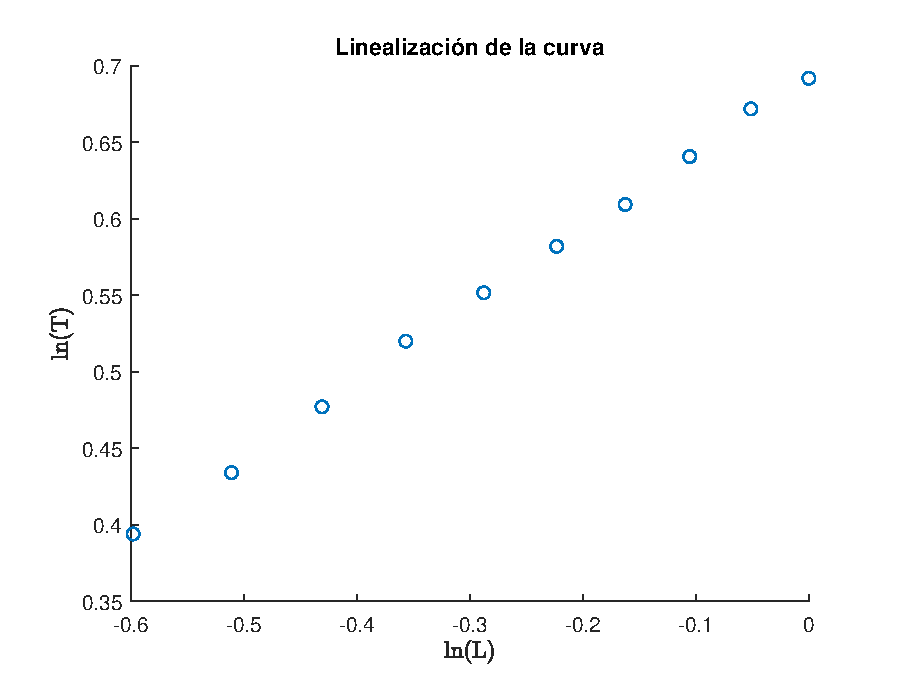
\includegraphics[width=0.80\textwidth]{resources/m1.2.eps}
\caption{Gráfica de $ln(L)$ vs. $ln(T)$.}
\label{figura3}
\source{Elaboración propia.}
\end{figure}

Se calculan los parámetros de la recta por el método de los mínimos cuadrados,
con la ayuda de los datos presentados en el \textbf{Cuadro \ref{cuadro5}}.

\begin{table}[!h]
\begin{center}
\begin{tabular}{|c|>{\centering}m{1.8cm}<{\centering}
                  |>{\centering}m{1.8cm}<{\centering}
                  |>{\centering}m{1.8cm}<{\centering}
                  |>{\centering}m{1.8cm}<{\centering}
                  |>{\centering}m{1.8cm}<{\centering}
                  |>{\centering}m{2.1cm}<{\centering}|}
\hline
$i$ & $x_i y_i$ & $x^2_i$ & $y^2_i$ & $Y$ & $d_i$ & $d^2_i (\num{1e-4})$ \tabularnewline \hline
 1 & -0.2356 & 0.3574 & 0.1553 & 0.3938 &  0.0002 & 0.0005 \tabularnewline \hline
 2 & -0.2217 & 0.2609 & 0.1884 & 0.4375 & -0.0035 & 0.1222 \tabularnewline \hline
 3 & -0.2056 & 0.1856 & 0.2277 & 0.4777 & -0.0006 & 0.0034 \tabularnewline \hline
 4 & -0.1855 & 0.1272 & 0.2704 & 0.5150 &  0.0050 & 0.2516 \tabularnewline \hline
 5 & -0.1587 & 0.0828 & 0.3042 & 0.5496 &  0.0020 & 0.0387 \tabularnewline \hline
 6 & -0.1299 & 0.0498 & 0.3386 & 0.5820 & -0.0001 & 0.0001 \tabularnewline \hline
 7 & -0.0990 & 0.0264 & 0.3712 & 0.6125 & -0.0033 & 0.1060 \tabularnewline \hline
 8 & -0.0675 & 0.0111 & 0.4103 & 0.6412 & -0.0006 & 0.0042 \tabularnewline \hline
 9 & -0.0345 & 0.0026 & 0.4511 & 0.6683 &  0.0033 & 0.1109 \tabularnewline \hline
10 &       0 &      0 & 0.4784 & 0.6941 & -0.0025 & 0.0602 \tabularnewline \hline
\end{tabular}
\caption{Valores para el método de mínimos cuadrados.}
\label{cuadro5}
\source{Elaboración propia.}
\end{center}
\end{table}

\begin{equation*}
    n = 10
\end{equation*}
\begin{equation*}
    \sum x_i = -2.7261
\end{equation*}
\begin{equation*}
    \sum y_i = 5.5719
\end{equation*}
\begin{equation*}
    \sum x^2_i = 1.1038
\end{equation*}
\begin{equation*}
    \sum y^2_i = 3.1956
\end{equation*}
\begin{equation*}
    \sum x_i y_i = -1.3378
\end{equation*}
\begin{equation*}
    \Delta_1 = n \sum x^2_i - \left( \sum x_i \right)^2 = 3.6067
\end{equation*}
\begin{equation*}
    \Delta_2 = n \sum y^2_i - \left( \sum y_i \right)^2 = 0.9104
\end{equation*}
\begin{equation*}
    A = \frac{\sum y_i \sum x^2_i - \sum x_i y_i \sum x_i}{\Delta_1} = 0.6941
\end{equation*}
\begin{equation*}
    B = \frac{n \sum x_i y_i - \sum x_i \sum y_i}{\Delta_1} = 0.5022
\end{equation*}
\begin{equation*}
    \sum d^2 = \num{6.9772e-5}
\end{equation*}
\begin{equation*}
    \sigma^2 = \frac{\sum d^2_i}{n-2} = \num{8.7215e-6}
\end{equation*}
\begin{equation*}
    \sigma_A = \sqrt{\frac{\sigma^2 \sum x^2_i}{\Delta_1}} = 0.0016
\end{equation*}
\begin{equation*}
    \sigma_B = \sqrt{\frac{\sigma^2 n}{\Delta_1}} = 0.0049
\end{equation*}

\begin{equation*}
    A = (0.6941 \pm 0.0016) [u]; 0.2354 \%
\end{equation*}
\begin{equation*}
    B = (0.5022 \pm 0.0049) [u]; 0.9791 \%
\end{equation*}

Siendo el coeficiente de correlación:

\begin{equation*}
    R = \frac{n \sum x_i y_i - (\sum x_i)(\sum y_i)}{\sqrt{\Delta_1 \Delta_2}} = 0.9996
\end{equation*}

La ecuación de la recta resultante es:

\begin{equation*}
    y = 0.6941 + 0.5022 x
\end{equation*}

A partir de los parámetros de recta $A$ y $B$, se calculan los parámetros $a$ y
$b$ de la curva original y sus errores por el método de propagación de errores:

\begin{equation*}
    a = e^{A} = e^{0.6941} = 2.0019
\end{equation*}
\begin{equation*}
    b = B = 0.5022
\end{equation*}
\begin{equation*}
    e_a = e^A e_A = e^{0.6941} 0.0016 = 0.0033
\end{equation*}
\begin{equation*}
    e_b = e_B = 0.0049
\end{equation*}

Obteniendo finalmente los valores de la curva:

\begin{equation*}
    a = (2.0019 \pm 0.0033) [u]; 0.1634 \%
\end{equation*}
\begin{equation*}
    b = (0.5022 \pm 0.0049) [u]; 0.9791 \%
\end{equation*}

La ecuación de la curva resultante es:

\begin{equation*}
    T = a L^b = 2.0019 d^{0.5022} = 2.0019 \sqrt{d}
\end{equation*}
\end{document}

